
\documentclass[11pt,a4paper]{article} %UKenglish,
\textheight24cm
\textwidth16cm
\topmargin-5mm
\oddsidemargin0cm
\evensidemargin0cm

\usepackage{enumerate}
\usepackage{textcomp}
\usepackage{url}
\usepackage{graphicx}
\usepackage[numbers]{natbib}
\usepackage{bussproofs}
\usepackage{tikz}
\usepackage{amssymb}
\usepackage{amsmath}
\usepackage{amsthm}
\usepackage{verbatim}
\usepackage{caption}
\usepackage{subcaption}
\usepackage[all,cmtip]{xy}
\usetikzlibrary{positioning, automata, shapes.geometric}
\usetikzlibrary{decorations.pathmorphing}
\usepackage{tikz-qtree}
 \usetikzlibrary{snakes, fit}
\usepackage[utf8]{inputenc}



\tikzset{snake it/.style={decorate, decoration=snake}}
\urlstyle{same}


\newcommand{\dftoutputlast}{\phi}
\newcommand{\xra}[1]{\overset{#1}{\rightsquigarrow}}

\newtheorem{lemma}{Lemma}
\newtheorem{theorem}{Theorem}
\newtheorem{definition}{Definition}
\newtheorem{example}{Example}
\newtheorem{corollary}{Corollary}


\begin{document}


\sloppy

\title{Rational index of the languages of bounded dimension\footnote{%
This research was supported by the Russian Science Foundation, project 18-11-00100.}}

\author{Ekaterina Shemetova\footnote{%
Department of Mathematics and Computer Science, St. Petersburg State University, 
7/9 Universitetskaya nab., Saint Petersburg 199034, Russia.}
\footnote{%
St. Petersburg Academic University, 
ul. Khlopina, 8, Saint Petersburg 194021, Russia.}
\footnote{%
JetBrains Research,
Primorskiy prospekt 68-70, Building 1, St. Petersburg, 197374, Russia.}
\and
Alexander Okhotin\footnotemark[2]
\and
Semyon Grigorev\footnotemark[2] \footnotemark[4]
}

\maketitle


\begin{abstract}
The rational index of a context-free language  $L$ is a function $f(n)$, such that for each regular language $R$ recognized by an automaton with $n$ states, the intersection of $L$ and $R$ is either empty or contains a word shorter than $f(n)$. It is known that the context-free language (CFL-)reachability problem and Datalog chain query evaluation for context-free languages (queries) with the polynomial rational index is in NL, while these problems is P-complete in the general case. We investigate the rational index of the languages of bounded dimension and show that it is of polynomial order. We obtain upper bounds on the values of the rational index for general languages of bounded dimension and for some of its previously studied subclasses.

\textbf{Keywords.}
Dimension of a parse tree; rational index; CFL-reachability; parallel complexity; context-free languages; Datalog programs.
\end{abstract}


\section{Introduction}
\label{intro}
The notion of a rational index was introduced by Boasson et al. \cite{RatBasic} as a complexity measure for context-free languages. The rational index $\rho_L(n)$ is a function, which denotes the maximum length of the shortest word in $L \cap R$, for arbitrary $R$ recognized by an $n$-state automaton. The rational index plays an important role in determining the parallel complexity of such practical problems as the context-free language (CFL-)reachability problem and Datalog chain query evaluation.

The CFL-reachability problem for a fixed context-free grammar $G$ is stated as follows: given a directed edge-labeled graph $D$ and a pair of nodes  $u$ and $v$, determine whether there is a path from $u$ to $v$ labeled with a string in $L(G)$. That is, CFL-reachability is a kind of graph reachability problem with path constraints given by context-free languages. It is an important problem underlying some fundamental static code analysis like data flow analysis and program slicing \cite{RepsBasic}, alias analysis \cite*{Chatterjee, alias}, points-to analysis \cite{Incremental} and other \cite{Cai, android, typeflow}, and graph database query evaluation \cite{Azimov, GrigorevRagozina, HellingsCFPQ, RDF}. The \textit{Datalog chain query} evaluation on a database graph is equivalent to the CFL-reachability problem \cite{10.1145/28659.28685, Ullman}. 


Unlike context-free language recognition, which is in NC (when context-free grammar is fixed), the CFL-reachability problem is P-complete \cite{ PCompl, RepSeq,  Yannakakis}. Practically, it means that there is no efficient parallel algorithm for solving this problem (unless P $\neq$ NC). 


The question on the parallel complexity of Datalog chain queries was investigated independently \cite{ChainQ, Vardi, Ullman}. Ullman and Van Gelder \cite{Ullman} introduce the notion of a \textit{polynomial fringe property} and show that chain queries having this property is in NC. The polynomial fringe property is equivalent to having the polynomial rational index: for a context-free language $L(G)$ having the polynomial rational index $\rho_L(n) = poly(n)$, where $poly(n)$ is some polynomial, is the same as for corresponding chain query to have the polynomial fringe property. It has been shown that for every algebraic number $\gamma$, a language with the rational index in $\Theta (n^\gamma )$ exists \cite{GreibRat}.  In contrast, the rational index of languages, which generate all context-free languages (an example of such language is the Dyck language on two pairs of parentheses $D_2$) is in order $exp(\Theta(n^2/\ln n))$ \cite{CFRat}, and, hence, this is the upper bound on the value of the rational index for every context-free language.


While both problems is not parallelizable in general, it is useful to develop more efficient parallel solutions for specific subclasses of the context-free languages. For example, there are context-free languages which admit more efficient parallel algorithms in comparison with the general case of context-free recognition \cite{IBARRA2, IBARRA, Okhotin2014ComplexityOI}.  The same holds for the CFL-reachability problem: there are some examples of context-free languages, for which the CFL-reachability problem lies in NL complexity class (for example, linear and one-counter languages) \cite{labelledGraphs, LReach, Regularrealizability, VyalyiRR}. These languages have the polynomial rational index.


The family of linear languages (linear Datalog chain programs, respectively) is the well-known subclass of context-free languages having the polynomial rational index \cite{RatBasic, Ullman}. The value of its rational index is in $O(n^2)$ \cite{RatBasic}. It is known that problems solvable by a linear Datalog Program are solvable in non-deterministic logarithmic space and, hence,  highly parallelizable. This class has received a lot of interest in complexity of constraint satisfaction, deductive databases and logic \cite{ linearisability, Dalmau2005LinearDA, linopt, Ullman}. 


In this work we investigate the rational index of the languages of bounded dimension, which are the natural generalization of the linear languages. The dimension of a parse tree considered as a measure of its branching. 


\textbf{Our contributions.} Our results can be summarized as follows:
\begin{itemize}
\item We show that the rational index of the languages of bounded dimension is polynomial and give an upper bound on its value in dependence of the value of dimension.
\item We give a lower bound on the rational index of the languages of bounded dimension, particularly we show that for any dimension $d$ there is a language of dimension $d$ that has the rational index is in $O(n^{2d})$.

\end{itemize}





\section{Preliminaries}
\label{sec:prel}
\label{preliminaries}
\paragraph{Formal languages.} 
A \textit{context-free grammar} is a 4-tuple $G = (\Sigma, N, P, S)$, where $\Sigma$ is a finite set of alphabet symbols,  $N$ is a set of nonterminal symbols, $P$ is a set of production rules and $S$ is a start nonterinal. $L(G)$ is a context-free language generated by context-free grammar $G$. We use the notation $A \stackrel {*}{\Rightarrow } w$  to denote that the string $w \in \Sigma^*$ can be derived from a nonterminal $A$ by sequence of applying the production rules from $P$. A \textit{parse tree} is an entity which represents the structure of the derivation of a terminal string from some nonterminal.


A grammar $G$ is said to be is in the \textit{Chomsky normal form}, if all production rules of $P$ are of the form:
$A \rightarrow BC$, $A \rightarrow a$ or $S \rightarrow \varepsilon$, where $A, B, C \in N$ and $a \in \Sigma$. 


The set of all context-free languages is identical to the set of languages accepted by pushdown automata (PDA). \textit{Pushdown automaton} is a 7-tuple $M = (Q, \Sigma, \Gamma, \delta, q_0, Z, F)$, where $Q$ is a finite set of states, $\Sigma$ is a input alphabet, $\Gamma$ is a finite set which is called the stack alphabet, $\delta$ is a finite subset of $Q \times (\Sigma \cap \{\varepsilon\}) \times \Gamma \times Q \times \Gamma^*$,
$q_{0}\in Q$ is the start state, $Z \in \Gamma$ is the initial stack symbol and
$F\subseteq Q$ is the set of accepting states.


A \textit{regular language} is a language that can be expressed with a regular expression or a deterministic or non-deterministic finite automata.
A \textit{nondeterministic finite automaton} (NFA) is represented by a 5-tuple, $(Q,\Sigma ,\delta ,Q_{0},F)$, where $Q$ is a finite set of states, $\Sigma$ is a finite set of input symbols, $\delta:Q\times \Sigma \rightarrow 2^{|Q|}$ is a transition function, $Q_0 \subseteq Q$ is a set of initial states, $F \subseteq Q$ is a set of accepting (final) states. \textit{Deterministic finite automaton} is a NFA with the following restrictions: each of its transitions is uniquely determined by its source state and input symbol, and reading an input symbol is required for each state transition.


 For a language $L$ over an alphabet $\Sigma$, its rational index $\rho_L$ is a function defined as follows:
$$\rho_L(n) = \max_{\mathcal{A} \text{:NFA with }n\text{ states}, L \cap L(\mathcal{A}) \neq \emptyset}\ \min_{w \in  L \cap L(\mathcal{A})}|w|.$$ 

\paragraph{Languages of bounded dimension.} 
For each node $v$ in a tree $t$, its dimension $dim(v)$ is inductively defined as follows:
\begin{itemize}
\item if $v$ is a leaf, then $dim(v)$ = 0
\item if $v$ is an internal node with $k$ children $v_1, v_2, ..., v_k$ for $k \ge 1$, then 
$$
dim(v) = 
 \begin{cases}
   \max_{i \in \{1...k\}}dim(v_i) &\text{if there is a unique maximum}\\
   \max_{i \in \{1...k\}}dim(v_i)+1 &\text{otherwise}
 \end{cases}
$$
\end{itemize}


The dimension of a parse tree $t$ $dim(t)$ is the dimension of its root. 
It is observable from the definition that the dimension of a tree $t$
is the height of the largest perfect binary tree,
which can be obtained from $t$ by contracting edges and accordingly identifying vertices.
A tree of dimension $dim(t) = 2$ is illustrated in Figure~\ref{oscbtree}.
\begin{figure}
\centering
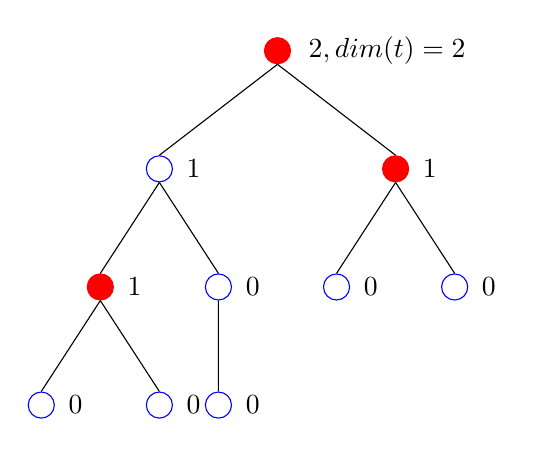
\begin{tikzpicture}[
level 1/.style={sibling distance=3cm},
level 2/.style={sibling distance=1.5cm}]
%\tikzstyle{every node}=[circle,draw]

\node[circle,draw] (Root) [ fill=red, red] {}
    child {
    node[circle,draw, blue] (l) {} 
    child { node[circle,draw, fill=red, red](ll) {}
            child { node[circle,draw, blue] (p) {} }
            child { node[circle,draw, blue] (pl) {} }
             }
    child { node[circle,draw, blue](lr) {} 
          child { node[circle,draw, blue] (plr) {} }
      }
}
child {
    node[circle,draw,  fill=red, red] (r) {}
    child { node[circle,draw, blue] (rl) {}} 
    child { node[circle,draw, blue] (rr) {} }
};
\node  [right=0.05cm of p] {0};
\node  [right=0.1cm of Root] {$2, dim(t)=2$};
\node  [right=0.05cm of l] {1};
\node  [right=0.05cm of r] {1};
\node  [right=0.05cm of ll] {1};
\node  [right=0.05cm of lr] {0};
\node  [right=0.05cm of pl] {0};
\node  [right=0.05cm of plr] {0};
\node  [right=0.05cm of rl] {0};
\node  [right=0.05cm of rr] {0};
\end{tikzpicture}
\caption{A tree $t$ with $dim(t)=2$. Nodes having children without unique maximum are filled.}
\label{oscbtree}            
\end{figure}

\begin{definition}[Grammars of bounded dimension]
Context-free grammar $G$ is of bounded dimension if the every parse tree $t$ of $G$ has $dim(t) \le d$, where $d$ is some constant. Then $d$ is called a dimension $dim(G)$ of $G$.
\end{definition}

\begin{definition}[Languages of bounded dimension]
Languages of bounded dimension are languages generated by grammars of bounded dimension. 
\end{definition}


\paragraph{Context-free language reachability.} 
A \textit{directed labeled graph} is a triple $D = (Q, \Sigma, \delta)$, where $Q$ is a finite set of nodes, $\Sigma$ is a finite set of alphabet symbols,
and $\delta \subseteq Q \times \Sigma \times Q$ is a finite set of labeled edges. Let $L(D)$ denote a graph language a regular language, which is recognized by the NFA $(Q,\Sigma ,\delta ,Q, Q)$ obtained from $D$ by setting every state as inial and accepting.


Let $i\pi j$ denote a unique path between nodes $i$ and $j$ of the input graph and $l(\pi)$ denote a unique string obtained by concatenating edge labels along the path $\pi$. Then the CFL-reachability can be defined as follows.
\begin{definition}[Context-free language reachability]
Let $L \subseteq \Sigma^*$ be a context-free language and $D = (Q, \Sigma, \delta)$ be a directed labeled graph. Given two nodes $i$ and $j$ we say that $j$ is \textit{reachable} from $i$ if there exists a path $i \pi j$, such that $l(\pi) \in L$. 
\end{definition}
There are four varieties of CFL-reachability problems: all-pairs problem, single-source problem, single-target problem and single-source/single-target problem \cite{RepsBasic}. In this paper we consider single-source/single-target problem. 



\section{Rational index of languages of bounded dimension}
\label{sec:osc}
\subsection{Upper bounds on the rational index of languages of bounded dimension}
Assume w.l.o.g. that considered context free-grammars is a CFGs in Chomsky normal form as this simplifies the notation. 


Before we estimate the value of the rational index for languages of bounded dimension, we need to prove the following.
\begin{lemma}
\label{lem:treeheight}
Let  $G = (\Sigma, N, P, S)$ be a context-free grammar in Chomsky normal form,  $D=(V, E, \Sigma)$ be a directed labeled graph with $n$ nodes. Let $w$ be the shortest string in $L(G)\cap L(D)$. Then the height of every parse tree for $w$ in $G$ does not exceed $|N|n^2$.
\end{lemma}

\begin{proof}
Consider grammar $G'$ for $L(G)\cap L(D)$. The grammar $G = (\Sigma, N', P', S')$ can be constructed from $G$ using the classical construction by Bar-Hillel et al.~\cite{BarHillel}: $N' \subseteq N \times V \times V $  contains all tiples $(A, i, j)$ such that $A \in N, i, j \in V$ ; $P'$ contains production rules in one of the following forms:
\begin{enumerate}
\item $(A, i, j) \rightarrow (B, i, k), (C, k, j)$ for all $(i, k, j)$ in $V$  if $A \rightarrow BC \in P$
\item $(A, i, j) \rightarrow a$ for all $(i, j)$ in $V$ if $A \rightarrow a$.
\end{enumerate}
A triple $(A, i, j)$ is \textit{realizable} if and only if there is a path $i\pi j$ such that $A \stackrel {*}{\Rightarrow } l(\pi)$ for some nontermimal $A \in N$. Then the parse tree $t_G$ for $w$ in $G$ can be converted into parse tree $t_{G'}$ in $G'$. Notice that every node of $t_{G'}$ is realizable triple. Also it is easy to see that the height of $t_G$ is equal to the height of $t_{G'}$. Assume that $t_{G'}$ for $w$ has a height of more than $|N|n^2$. Consider a path from the root of the parse tree to a leaf, which has length greater than $|N|n^2$. There are $|N|n^2$ unique labels $(A, i, j)$ for nodes of the parse tree, so according to the pigeonhole principle, this path has at least two nodes with the same label. This means that the parse tree for $w$ contains at least one subtree $t$ with label $(A, i, j)$ at the root, which has a subtree $t'$ with the same label. Then we can change $t$ with $t'$ and get a new string $w'$ which is shorter than $w$, because the grammar is in Chomsky normal form. But $w$ is the shortest, then we have a contradiction.
\end{proof}
From Lemma~\ref{lem:treeheight} one can deduce an alternative proof of the fact that the rational index of linear languages is in $O(n^2)$ \cite{RatBasic}: the number of leaves in a parse tree in linear grammar in Chomsky normal form is proportional to its height, and thus it is in $O(n^2)$.
\begin{theorem}
\label{oscbnddim}
Let $G = (\Sigma, N, P, S)$ be a grammar in Chomsky normal form with dimension $dim(G)=d$. Let $0 \leq d \leq c$, where $c$ is some constant, $A \in N$, $\mathcal{A}$ --- NFA with $n$ states, where $p$ and $q$ is a start and final state respectively, and let $w$ be the shortest string having a parse tree with root labeled by $A$. Suppose that there is a computation path $p \xra{w} q$ in $\mathcal{A}$. Then $|w| \leq |N^d|n^{2d}$.
\end{theorem}
\begin{proof}
Proof by induction on $dim(G)$.

\textbf{Basis.} $dim(G) = 0$.
\\
Consider the grammar $G_0$ with $dim(G_0) = 0$. $dim(G_0)=0$ if $G_0$ has single rule of the form $S \rightarrow a$, where $a \in \Sigma$. Clearly, $|w| = 1 \leq |N| n^0 = |N|$.

\textbf{Inductive step.} $dim(G) = d$.
\\
Let $d \ge 1$, then $A \rightarrow BC \in P$. Let $w=uv$, where $B  \stackrel {*}{\Rightarrow } u$ and $C  \stackrel {*}{\Rightarrow } v$. Let $t_1$ and $t_2$ are parse trees for $u$ and $v$ respectively. By the definition of the dimension there are two cases:
\begin{enumerate}
\item $dim(t_1) = dim(t_2) = d-1$ (Figure~\ref{dimupper:1}). Since $w$ is the shortest, then $u$ and $v$ are the shortest, and the computation for $w$ can be factorized as $p \xra{w} q = p \xra{u} r \xra{v} q$. By the induction hypothesis, $|u|, |v| \leq |N|^{d-1} n^{2(d-1)}$. Then $|w| \leq 2|N|^{d-1} n^{2(d-1)} \leq |N|^d n^{2d}$.
\item $dim(t_1) < d$ and $dim(t_2) = d$  (Figure~\ref{dimupper:2}). Then $w$ can be factorized as $w = v_l v_{l-1} ...v_1 v_0$, where parse tree for $v_i$ has dimension $d-1$ in the worst case. By the induction hypothesis, $|v_i| \leq |N|^{d-1}n^{2(d-1)}$ for all $i$ and by Lemma~\ref{lem:treeheight} $w = \sum_i |v_i| \leq l |N|^{d-1}n^{2(d-1)} \leq h |N|^{d-1}n^{2(d-1)} \leq |N|n^2 |N|^{d-1}n^{2(d-1)} = |N|^d n^{2d}$.

Case $dim(t_2) < d$ and $dim(t_1) = d$ can be proved symmetrically.
\end{enumerate}
\end{proof}



\begin{figure}
\centering
\begin{subfigure}{.5\textwidth}
  \centering
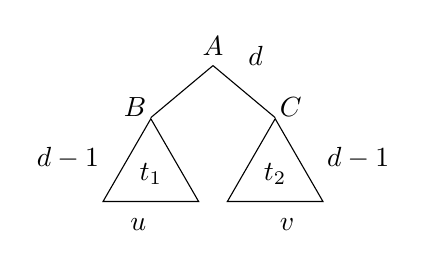
\begin{tikzpicture}[level distance = 45pt, sibling distance = 10pt]
  \tikzset{every leaf node/.style = {draw, regular polygon, regular polygon sides = 3, inner sep = 3pt}}

  \Tree [.$A$
        $t_1$
        $t_2$
      ] 
\node (root) [] {};
\node  (l2) [below=0.4cm of root] {};
\node  (d) [right=0.2cm of root] {$d$};
\node  [right=0.6cm of l2] {$C$};
\node  [left=0.6cm of l2] {$B$};
\node  (l4) [below=0.4cm of l2] {};
\node  [right=1.2cm of l4] {$d-1$};
\node  [left=1.2cm of l4] {$d-1$};
\node  (l3) [below=1.9cm of root] {};
\node  [right=0.6cm of l3] {$v$};
\node  [left=0.6cm of l3] {$u$};
\end{tikzpicture}
  \caption{$dim(t_1) = dim(t_2) = d-1$}
  \label{dimupper:1}
\end{subfigure}%
\begin{subfigure}{.5\textwidth}
  \centering
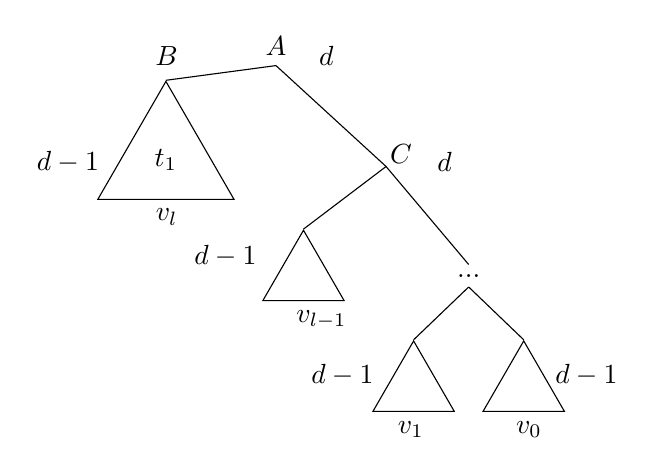
\begin{tikzpicture}[level distance = 40pt, sibling distance = 10pt]
  \tikzset{every leaf node/.style = {draw, regular polygon, regular polygon sides = 3, inner sep = 6pt}}

\Tree [.$A$ $t_1$ 
                                                     [$$ [.$...$ $$  $$ ] ] ]
           ]
\node (root) [] {};
\node  (l2) [below=0.07cm of root] {};
\node  (a) [left=1cm of root] {$B$};
\node  (l3) [below=1cm of root] {};
\node  (b) [right=1.2cm of l3] {$C$};
\node  (l4) [below=3.1cm of root] {};
\node  (c) [right=0.01cm of l4] {$v_{l-1}$};
\node  (l5) [below=1.8cm of root] {};
\node  (d) [left=1cm of l5] {$v_l$};
\node  (l6) [below=4.5cm of root] {};
\node  (e) [right=1.3cm of l6] {$v_1$};
\node  (f) [right=2.8cm of l6] {$v_0$};
\node  (l7) [below=1.1cm of root] {};
\node  (g) [left=2cm of l7] {$d-1$};
\node  (k) [right=0.3cm of root] {$d$};
\node  (j) [right=1.8cm of l7] {$d$};
\node  (l8) [below=2.3cm of root] {};
\node  (l) [left=0.001cm of l8] {$d-1$};
\node  (l9) [below=3.8cm of root] {};
\node  (m) [right=0.2cm of l9] {$d-1$};
\node  (n) [right=3.3cm of l9] {$d-1$};
\end{tikzpicture}
  \caption{$dim(t_1) = d-1$ and $dim(t_2) = d$}
  \label{dimupper:2}
\end{subfigure}
\caption{Two cases for the dimensions of children of the root}
\label{dimupper}
\end{figure}

\label{sec:osc_lower}
\subsection{Lower bounds on the rational index of languages of bounded dimension}
\begin{theorem} Let $G = (\Sigma, N, P, S)$ be a grammar of bounded dimension $dim(G) = d$, where $d$ is some constant. Then there exists a language $L(G)$ with rational index in $O(n^{2d})$ for any $n$.
\begin{proof} Graph and grammar can be constructed inductively on $dim(G)$.

\textbf{Basis.} $dim(G) = 1$.

The family of the languages having dimension $d = 1$  coincides with the family of linear languages. Consider a linear grammar $G_1=(\{a, b\}, \{S\}, \{S \rightarrow aSb\ |ab\}, S)$ which generates a language $L(G_1) = \{a^kb^k \vert k > 0\}$. 
Consider a NFA $\mathcal{A}_1$ consisiting of two cycles connected via a shared node $q_0$ (Figure~\ref{worstd_1}). Suppose the first cycle consists of $m$ edges labeled with $a$, and the second cycle consists of $m'$ edges labeled with $b$. 
Let $m$ and $m'$ be coprime integers, and let $q_0$ be start and final state of $\mathcal{A}_1$. Then the length of the shortest word $w \in L(G_1) \cap L(\mathcal{A}_1)$ equals $2mm'$. Suppose $\mathcal{A}_1$ has $n$ states, and let $m = n/2 + 1$, $m'=n/2$. It is easy to see that $m$ and $m'$ are coprime for all $n$. Then $|w| = 2mm' = 2n/2(n/2 + 1) = O(n^2) = O(n^{2d})$. This example is well-known to the community~\cite{HellingsCFPQ, Yannakakis}. 

\begin{figure}[h]
    \centering        
    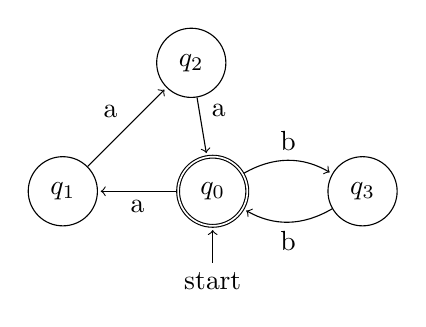
\begin{tikzpicture}[shorten >=1pt,auto]
       \node[state] (q_0)                      {$q_1$};
       \node[state] (q_1) [above right=of q_0] {$q_2$};
       \node[state,  initial below, accepting] (q_2) [right=of q_0]       {$q_0$};
       \node[state] (q_3) [right=of q_2]       {$q_3$};
        \path[->]
        (q_0) edge  node {a} (q_1)
        (q_1) edge   node {a} (q_2)
        (q_2) edge  node {a} (q_0)
        (q_2) edge[bend left, above]  node {b} (q_3)
        (q_3) edge[bend left, below]  node {b} (q_2);
    \end{tikzpicture}

\caption{Worst-case NFA $\mathcal{A}_1$ for $L(G_1)$ and $n=4$ ($m = 3, m' = 2$). }
\label{worstd_1}
\end{figure}

\textbf{Inductive step.} $dim(G) = d$.

Let $G_{d-1} =  (\Sigma_{d-1}, N_{d-1}, P_{d-1}, S_{d-1})$ be a context-free grammar with $dim(G_{d-1}) = d-1$ and $\mathcal{A}_{d-1}= (Q_{d-1},\Sigma_{d-1} ,\delta_{d-1} ,q^{d-1}_{0},\{q^{d-1}_{0}\})$  be a NFA with $n$ states. Let $w_0^{d-1}$ be the shortest string in $L(G_{d-1}) \cap L(\mathcal{A}_{d-1})$.

\textit{Construction of the grammar $G_d = (\Sigma_{d}, N_{d}, P_{d}, S_{d})$}. Grammar $G_d$ can be defined as follows:
\begin{itemize}
\item $\Sigma_{d} = \Sigma_{d-1} \cup \{a_d, b_d, c_d\}$
\item $P_{d} = P_{d-1} \cup P'$, where $P' = 
\{ 
\\ S_d \rightarrow A_d S_d c_d\ \vert \ A_d c_d
\\ A_d \rightarrow a_d A_d b_d\ \vert \ a_d S_{d-1}  b_d
\\  \}$. 
\item $N_d = N_{d-1} \cup \{S_d, A_d\}$. 
\end{itemize}
It is left to show that dimension $dim(G_d) = dim(G_{d-1}) + 1 = d$. Consider the dimension of the parse tree $t$ labeled by $A_d$ (Figure~\ref{dimsubtree:1}). By the induction $dim(S_{d-1}) = d-1$. It is easy to see that dimension of $dim(t) = dim(G_{d-1}) = d-1$. Multiple applications of the rule $A_d \rightarrow a_d A_d b_d$ do not increase the dimension of the parse tree because the dimensions of nodes labeled with $a_d$, $b_d$ are equal to $0$.


Now consider the dimension of the parse tree $t$ labeled by $S_d$ (Figure~\ref{dimsubtree:2}). As it was mentioned above, nodes labeled with $A_d$ have dimension $d -1$, nodes labeled with $S_d$ have dimension $d -1$ and  nodes labeled with $c_d$ have dimension $0$. As there is no unique maximum, $dim(t) = \max_{i} (v_i) + 1 = d - 1 + 1 = d$. Notice that only one application of the rule  $S_d \rightarrow A_d S_d c_d$ increases the dimension of $t$, whereas futher applications do not make any effect on the dimension of parse tree.

\begin{figure}
\centering
\begin{subfigure}{.5\textwidth}
  \centering
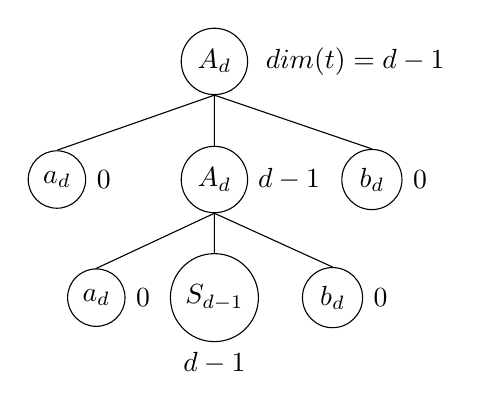
\begin{tikzpicture}[
level 1/.style={sibling distance=2cm},
level 2/.style={sibling distance=1.5cm}]
%\tikzstyle{every node}=[circle,draw]

\node[circle,draw] (Root) [ ] {$A_d$}
    child {
    node[circle,draw] (1) {$a_d$} 
}
child{ node[circle,draw] (2) {$A_d$} child[circle,draw] {node[circle,draw]  (3) {$a_d$}} child{node[circle,draw]  (4) {$S_{d-1}$}}
  child {
    node[circle,draw] (5) {$b_d$} 
   }
}
child {
    node[circle,draw] (6) {$b_d$}};
\node  [right=0.1cm of Root] {$dim(t)=d-1$};
\node  [right=0.01cm of 1] {$0$};
\node  [right=0.001cm of 2] {$d-1$};
\node  [right=0.01cm of 3] {$0$};
\node  [below=0.001cm of 4] {$d-1$};
\node  [right=0.01cm of 5] {$0$};
\node  [right=0.01cm of 6] {$0$};
\end{tikzpicture}
  \caption{Parse tree labeled with $A_d$}
  \label{dimsubtree:1}
\end{subfigure}%
\begin{subfigure}{.5\textwidth}
  \centering
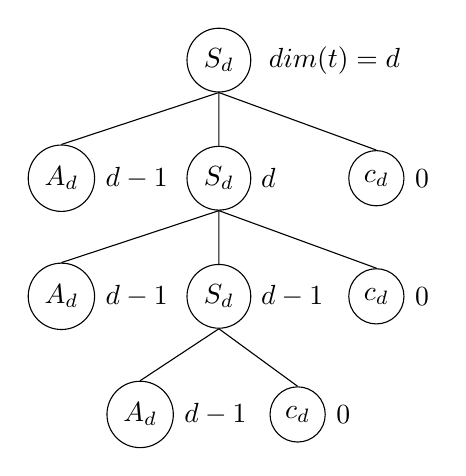
\begin{tikzpicture}[
level 1/.style={sibling distance=2cm},
level 2/.style={sibling distance=2cm}]
%\tikzstyle{every node}=[circle,draw]

\node[circle,draw] (Root) [ ] {$S_d$}
    child {
    node[circle,draw] (1) {$A_d$} 
}
child{ node[circle,draw] (2) {$S_d$} child[circle,draw] {node[circle,draw]  (3) {$A_d$}} child{node[circle,draw]  (4) {$S_{d}$} child[circle,draw] {node[circle,draw]  (7) {$A_d$}} child[circle,draw] {node[circle,draw]  (8) {$c_d$}} }
  child {
    node[circle,draw] (5) {$c_d$} 
   }
}
child {
    node[circle,draw] (6) {$c_d$}};
\node  [right=0.1cm of Root] {$dim(t)=d$};
\node  [right=0.01cm of 1] {$d-1$};
\node  [right=0.001cm of 2] {$d$};
\node  [right=0.01cm of 3] {$d-1$};
\node  [right=0.001cm of 4] {$d-1$};
\node  [right=0.01cm of 5] {$0$};
\node  [right=0.01cm of 6] {$0$};
\node  [right=0.01cm of 7] {$d-1$};
\node  [right=0.01cm of 8] {$0$};
\end{tikzpicture}
  \caption{Parse tree labeled with $S_d$}
  \label{dimsubtree:2}
\end{subfigure}
\caption{Parse trees of $G_d$ and dimensions of their vertices}
\label{dimsubtree}
\end{figure}

\textit{Construction of NFA $\mathcal{A}_{d} = (Q_d,\Sigma_d ,\delta_d ,q^{d}_{0},F_d$)} with $n$ vertices. 

Suppose w.l.o.g. that $n$ is divisible by $4$.
Assume that the number of states in NFA $\mathcal{A}_{d-1}= (Q_{d-1},\Sigma_{d-1} ,\delta_{d-1} ,q^{d-1}_{0},\{q^{d-1}_{0}\})$ equals to $n/2$ (by the induction hypothesis such an automaton exists). Fix two coprime integers $m=n/4 + 1$ and $m' = n/4$.

Then NFA $\mathcal{A}_{d}$ can be defined as follows:
\begin{itemize}
\item $\Sigma_{d} = \Sigma_{d-1} \cup \{a_d, b_d, c_d\}$
\item $\delta_{d} = \delta_{d-1} \cup \{
\\(q^{d}_{0}, a_d) \rightarrow q^{d-1}_{0},
\\(q^{d-1}_{0}, b_d) \rightarrow q^{d}_{1},
\\(q^{d}_{i}, b_d) \rightarrow q^{d}_{i+1}, 1 \le i \le m-1,
\\(q^{d}_{i}, a_d) \rightarrow q^{d}_{i-1}, 1 \le i \le m-1,
\\(q^{d}_{m-1}, b_d) \rightarrow q^{d}_{0},
\\(q^{d}_{0}, c_d) \rightarrow p^{d}_{1},
\\(p^{d}_{i}, c_d) \rightarrow p^{d}_{i+1}, 1 \le i \le m'-1,
\\(p^{d}_{m'-1}, c_d) \rightarrow q^{d}_{0}\}$
\item $F_d = \{q^{d}_{0}\}$
\item $Q_d = Q_{d-1} \cup \{ q^d_{0}, ..., q^d_{m-1}, p^d_{0}, ..., p^d_{m'-1}\}$
\end{itemize}
The general form of $\mathcal{A}_{d}$ is shown in Figure~\ref{dimautomata:generalized}.

Let $w$ be the shortest sting in $L(G_d) \cap L(\mathcal{A}_{d})$. Consider how $w$ is formed. Start state is $q^{d}_{0}$. According to the grammar rule $S_d \rightarrow A_d S_d c_d\ \vert \ A_d c_d $, $w$ should start from a substring $u$ such that $A_d  \stackrel {*}{\Rightarrow } u$. There is the only one outgoing edge labeled with $a_d$, so the next state is $q^{d-1}_{0}$. The next part of $w$ should be a symbol $a_d$  or a word $v$ such that $S_{d-1}  \stackrel {*}{\Rightarrow } u$. As there is no outgoing edge labeled with $a_d$, $u$ is the shortest string in $L(G_d) \cap L(\mathcal{A}_{d-1})$, and, hence, $u = w_0^{d-1}$. Now the first part of $w$ is $a_d w_0^{d-1}$. To complete a substring derived by $A_d$, there is only one possible transition, which is an edge from $q^{d-1}_{0}$ to $q^d_1$ labeled with $b_d$. The next substring should be symbol $c_d$ (the rule $S_d \rightarrow A_d c_d$) or a word derived by $A_d$. The only suitable transition here is an edge from $q^d_1$ to $q^{d-1}_{0}$ labeled by $a_d$, so the substring derived by $A_d$ is started. Again, to complete the word generated by $A_d$, one goes to the state $q^d_2$, and $w$ now starts with $a_d w_0^{d-1} b_d a_d a_d w_0^{d-1} b_d b_d$. By the construction of NFA $\mathcal{A}_{d}$, this process continues until one comes to the state $q^d_{0}$ without starting a substring derived by $A_d$ (notice that such substrings are the shortest possible). It happens after $m$ iterations. Then it is left to read $m$ symbols $c_d$ by going from $q^d_{0}$ to $q^d_{0}$. But $m$ and $m'$ are coprime, so to balance the number of substrings derived by $A_d$ and the number of symbols $c_d$, one needs to repeat the first cycle $m'$ times and the second cycle $m$ times.

Now estimate the length of $w$. Let $w_i$ be the shortest string such that there exists computation $q^{d}_{i-1} \xra{w_i} q^d_i$ ($q^{d}_{m-1} \xra{w_m} q^d_0$ for $w_m$) for $1\leq i \leq m$ in $\mathcal{A}_{d}$ and $A_d  \stackrel {*}{\Rightarrow }  w_i$. Notice that $w_i = a_d w_{i-1} b_d$ and $w_0 = w_0^{d-1}$, and there exists computation $q^{d}_{0} \xra{w_1} q^d_1  \xra{w_2} q^d_2 \xra{w_3} ... \xra{w_{m-1}} q^{d}_{m} \xra{w_m} q^d_0$ in $\mathcal{A}_{d}$.

Considering the above and the rules of the grammar $G_d$ $S_d \rightarrow A_dS_dc_d\vert A_dc_d$, $w$ is of the following form:

$$w = ({\prod_{i=1}^m w_i})^{m'}{c}_d^{mm'}$$

Then the length of $w$ can be calculated as follows:
$$|w| = ({\sum_{i=1}^m |w_i|})m' + mm' = (\sum_{i=1}^m (|w_0^{d-1}| + 2i))m' + mm'  = 
(\sum_{i=1}^m |w_0^{d-1}| + \sum_{i=1}^m 2i)m' + mm' = $$
$$ =  |w_0^{d-1}| m m' + 2mm' + (m-1)mm' + mm' = |w_0^{d-1}| m m' + 3mm' + (m-1)mm'.
$$
As the NFA $\mathcal{A}_{d-1}$ has $n/2$ states, by the induction assumption $|w_0^{d-1}| =O( (n/2)^{2d - 2})$. Recall that $m = n/4 +1$ and $m' = n/4$. Then the length of $w$ is equal to:
$$|w| = O((n/2)^{2d - 2}) (n/4 + 1) n/4 + 3(n/4 + 1) n/4 + (n/4 + 1) n^2/16  =$$ $$= O((n/2)^{2d - 2}) n^2/16 = O(n^{2d}).$$

Let $n = 2^k$, where $k > 0$ is some constant.

For $d=1$ let $m = 2^{k-1} + 1$ and $m'= 2^{k-1}$.  Then $|w| = 2^k(2^{k-1} + 1) \ge 2^{2k-1}$.

For $d=2$ let $m = 2^{k-2} + 1$ and $m'= 2^{k-2}$.  Then $|w| \ge 2^{2k-3} (2^{k-2} + 1)2^{k-2} \ge 2^{4k - 7}$.

Suppose that $|w| \ge 2^{2k(d-1)-c}$ for $d-1$ and some constant $c > 0$. Then for $dim = d$ $|w| \ge 2^{2(k-1)(d-1)-c}(2^{k-2}+1)2^{k-2} \ge 2^{2k-4+2kd-2k-2d+2-c} = 2^{2kd-2d-2-c} = 2^{2kd - c'}$, where $c' = c + 2d + 2$.
\end{proof}
\end{theorem}
\begin{figure}
\centering
\begin{minipage}{.5\textwidth}
  \centering
     \begin{tikzpicture}[shorten >=1pt,auto]
       \node[state] (q_10) [right=of q_0]       {$q^{d-1}_0$};
       \node[state, initial below, accepting] (q_20) [below right=of q_10]       {$q^d_0$};
      \node[state] (q_21) [below left=of q_10]       {$q^d_1$};
      \node[state] (q_22) [below=of q_21]       {$q^d_2$};
      \node (q_23) [below=of q_22]       {$...$};
      \node [state]  (q_24) [below=of q_23]       {$q^d_{m-1}$};
      \node[state] (p_21) [right=of q_20]       {$p^d_1$};
      \node (p_22) [below=of p_21]       {$...$};
      \node[state] (p_23) [below=of p_22]       {$p^d_{m'-1}$};
       \node  (l1) [right=1.1cm of q_21] {};
       \node  (m) [below=0.7cm of l1] {$m$};
       \node  (m') [right=2.5cm of m] {$m'$};
      \node (l2) [left=0.6cm of q_10]  {};
      \node (A) [above=1cm of l2]  {$\mathcal{A}_{d-1}$};
      \node (a) [left=of q_10]  {};
      \node (b) [right=of q_10]  {};
      \node (c) [above=of q_10]  {};
      \node [draw, inner sep=0.1cm, fit= (a) (q_10) (b) (c)] {};
        \path[->]
        (q_20) edge[below]  node {$a_d$} (q_10)
        (q_10) edge[below]  node {$b_d$} (q_21)
        (q_21) edge[above]  node {$a_d$} (q_20)
        (q_21) edge[bend left]  node {$b_d$} (q_22)
        (q_22) edge[bend left]  node {$a_d$} (q_21)
        (q_22) edge[bend left]  node {$b_d$} (q_23)
        (q_23) edge[bend left]  node {$a_d$} (q_22)
        (q_23) edge[bend left]  node {$b_d$} (q_24)
        (q_24) edge[bend left]  node {$a_d$} (q_23)
        (q_24) edge[]  node {$b_d$} (q_20)
        (q_20) edge[ above]  node {$c_d$} (p_21)
        (p_21) edge[]  node {$c_d$} (p_22)
        (p_22) edge[]  node {$c_d$} (p_23)
        (p_23) edge[]  node {$c_d$} (q_20);
    \end{tikzpicture}
  \captionof{figure}{NFA $\mathcal{A}_{d}$}
  \label{dimautomata:generalized}
\end{minipage}%
\begin{minipage}{.5\textwidth}
  \centering
     \begin{tikzpicture}[shorten >=1pt,auto]
       \node[state] (q_11)                      {$q^1_1$};
       \node[state] (q_12) [above right=of q_0] {$q^1_2$};
       \node[state] (q_10) [right=of q_0]       {$q^1_0$};
       \node[state] (p_11) [right=of q_2]       {$p^1_1$};
       \node[state, initial below, accepting] (q_20) [below right=of q_10]       {$q^2_0$};
      \node[state] (q_21) [below left=of q_10]       {$q^2_1$};
      \node[state] (q_22) [below=of q_21]       {$q^2_2$};
      \node[state] (p_21) [right=of q_20]       {$p^2_1$};
        \path[->]
        (q_10) edge  node {$a_1$} (q_11)
        (q_11) edge   node {$a_1$} (q_12)
        (q_12) edge  node {$a_1$} (q_10)
        (q_10) edge[bend left, above]  node {$b_1$} (p_11)
        (p_11) edge[below]  node {$b_1$} (q_10)
        (q_20) edge[below]  node {$a_2$} (q_10)
        (q_10) edge[below]  node {$b_2$} (q_21)
        (q_21) edge[above]  node {$a_2$} (q_20)
        (q_21) edge[bend left]  node {$b_2$} (q_22)
        (q_22) edge[bend left]  node {$a_2$} (q_21)
        (q_22) edge[below]  node {$b_2$} (q_20)
        (q_20) edge[bend left, above]  node {$c_2$} (p_21)
        (p_21) edge[bend left, below]  node {$c_2$} (q_20);
    \end{tikzpicture}
  \captionof{figure}{NFA $\mathcal{A}_{2}$ with $n=8$ and $m = 3, m' = 2$}
  \label{dimautomata:2}
\end{minipage}
\end{figure}
\begin{example}{}
The automaton $\mathcal{A}_{2}$ with $n = 8$ states, $m = 3$ and $m' = 2$ is illustrated in Figure~\ref{dimautomata:2}, the rules of the grammar $G_2$ : $\{  S_2 \rightarrow A_2S_2c_2\vert A_2c_2; A_2 \rightarrow a_2A_2b_2 \vert  a_2S_1b_2; S_1 \rightarrow a_1S_1b_1 \vert a_1b_1\}$.
\end{example}



\begin{subsection}{The rational indices of some subclasses of languages of bounded dimension}  



\paragraph{Superlinear languages.} 
A context-free grammar $G = (\Sigma, N, P, S)$ is \textit{superlinear} \cite{superlinear} if all productions of $P$ satisfy these conditions:
\begin{enumerate}
\item there is a subset $N_L \subseteq N$ such that every $A \in N_L$ has only linear productions $A\rightarrow aB$ or $A\rightarrow Ba$, where $B \in N_L$ and $a \in \Sigma$.
\item if $A \in N \setminus N_L$, then $A$ can have non-linear productions of the form $A \rightarrow BC$ where $B\in N_L$ and $C \in N$, or linear productions of the form $A\rightarrow \alpha B$ $\vert$ $B \alpha$ $\vert$ $\alpha$ for $B \in N_L$, $\alpha \in \Sigma^*$.
\end{enumerate}
A language is \textit{superlinear} if it is generated by some superlinear grammar. 
\begin{theorem} Let $G$ be a superlinear grammar. Then $\rho_{L(G)}$ is in $O(n^4)$.
\end{theorem}
\begin{proof}
From the definition of superlinear grammar $G$ it is observable that its parse trees have dimension at most 2. From 
Theorem~\ref{oscbnddim}, if dimensions of all parse trees are bounded by some $k$ then the rational index $\rho_{L(G)}$ of such language is in $O(n^4)$.
\end{proof}


\paragraph{Bounded-oscillation languages}
 Bounded-oscillation languages were introduced by Ganty and Valput \cite{BoundOsc} as the generalization of the class of linear languages. 

Oscillation is defined using a hierarchy of \textit{harmonics}. Let $\bar{a}$ be a \textit{push}-move and $a$ be a \textit{pop}-move. Then a PDA run $r$ can be described by a well-nested sequence $\alpha(r)$ of $\bar{a}$-s and $a$-s. Two positions $i<j$ form a \textit{matching pair} if the corresponding $\bar{a}$ at $i$-th position of the sequence matches with $a$ at $j$-th position. For example, word $\bar{a}\bar{a}\bar{a}aa\bar{a}aa$ has the following set of matching pairs: $\{(1, 8), (2, 5), (3, 4), (6, 7)\}$ ($\bar{a}(\bar{a}(\bar{a}a)a)(\bar{a}a)a$).


Harmonics are inductively defined as follows:
\begin{itemize}
\item  order 0 harmonic $h_0$ is $\varepsilon$
\item  $h_{(i+1)}$ harmonic is $\bar{a}h_ia\ \bar{a}h_ia$.
\end{itemize}

PDA run $r$ is \textit{k-oscillating} if the harmonic of order $k$ is the greatest harmonic that occurs in $r$ after removing $0$ or more matching pairs. 

\begin{definition}[Bounded-oscillation languages]
Bounded-oscillation languages are languages accepted by pushdown automata with all runs $k$-oscillating. 
\end{definition}
It is important that the problem whether a given CFL is a bounded-oscillation language is undecidable \cite{BoundOsc}.

The oscillation of a parse tree of a context-free grammar can be defined similarly to the oscillation of a PDA run. Given a parse tree $t$, we define corresponding well-nested word $\alpha(t)$ inductively as follows:
\begin{itemize}
\item if $n$ is the root of $t$ then $\alpha(t) = \bar{a}\alpha(n)$
\item if $n$ is a leaf then $\alpha(n)=a$
\item if $n$ has $k$ children then $\alpha(n) = a\underbrace{\bar{a}...\bar{a}}_\text{$k$ times}\alpha(n_1)...\alpha(n_k)$
\end{itemize}


Moreover, given a PDA run $r$, there exists a corresponding parse tree $t$ with the same well-nested word $\alpha(t)=\alpha(r)$ and vice versa \cite{BoundOsc}. Therefore, a language $L$ is of bounded oscillation if all parse trees in a corresponding context-free grammar have bounded oscillation.


The oscillation of a parse tree is closely related with its dimension. 
It is known that the dimension of parse trees and its oscillation are in linear relationship.

\begin{lemma}[\cite{BoundOsc}]
\label{boscdim}
Let a grammar $G = (\Sigma, N, P, S)$ be in Chomsky normal form and let $t$ be a parse tree of $G$. Then $osc(t) - 1 \le dim(t) \le 2osc(t)$.
\end{lemma}
Combining Theorem~\ref{oscbnddim} and Lemma~\ref{boscdim} we obtain the following.
\begin{corollary}
Let $L$ be a $k$-bounded-oscillation language. Then $\rho_{L(G)}$ does not exceed $O(n^{4k})$.
\end{corollary}



\end{subsection}

\section{Conclusion and open problems}
\label{sec:conc}

We have proved that bounded-oscillation languages
have polynomial rational index.
This means that the CFL-reachability problem and Datalog query evalution for these languages is in NC.
This class is a natural generalization of linear languages,
and might be the largest class of queries among such generalizations
that is known to be in NC.


There is a family of languages which has polynomial rational index,
but is incomparable with the linear languages:
\emph{the one-counter languages}.
Moreover, it is not comparable with the bounded-oscillation languages:
for example, the Dyck language $D_1$ is a one-counter language,
but not a bounded-oscillation language for any $k$.
Could this class be generalized in the same manner as linear languages
with respect to the polynomiality of the rational index?
One can consider the Polynomial Stack Lemma by Afrati et al.~\cite{ChainQ},
where some restriction on the PDA stack contents are given,
or investigate the properties of the substitution closure of the one-counter languages,
which is known to have polynomial rational index \cite{RatBasic}. 


%%For cite command type as \cite{1}; \cite{3,6} and \cite{2,4,6}.
%%For refcite command type as Refs.~[\refcite{1}];
%%[\refcite{1},\refcite{3}] and [\refcite{1}--\refcite{4}].


\begin{comment}
\section*{Acknowledgments}
This research was supported by the Russian Science Foundation, grant \textnumero 18-11-00100.
\end{comment}


\bibliographystyle{plain}
\bibliography{paper}
\end{document}